\chapter{Analyse performance}
\label{chapter-4}

%Résultats du calcul de la puissance reçue et du débit binaire dans l'appart

%Suggestions placement


\section{Résultats}

Les résultats ont été réalisés avec la simulation à sa plus haute résolution (soit des cellules de $0,0625\mathrm{m}\times0,0625\mathrm{m}$).

\subsection{Emplacement par défaut (salon)}
La station de base se trouve en (9,4 ; 7)m.

\subsubsection{Sans ascenseur}

\begin{figure}[H]
    \centering
    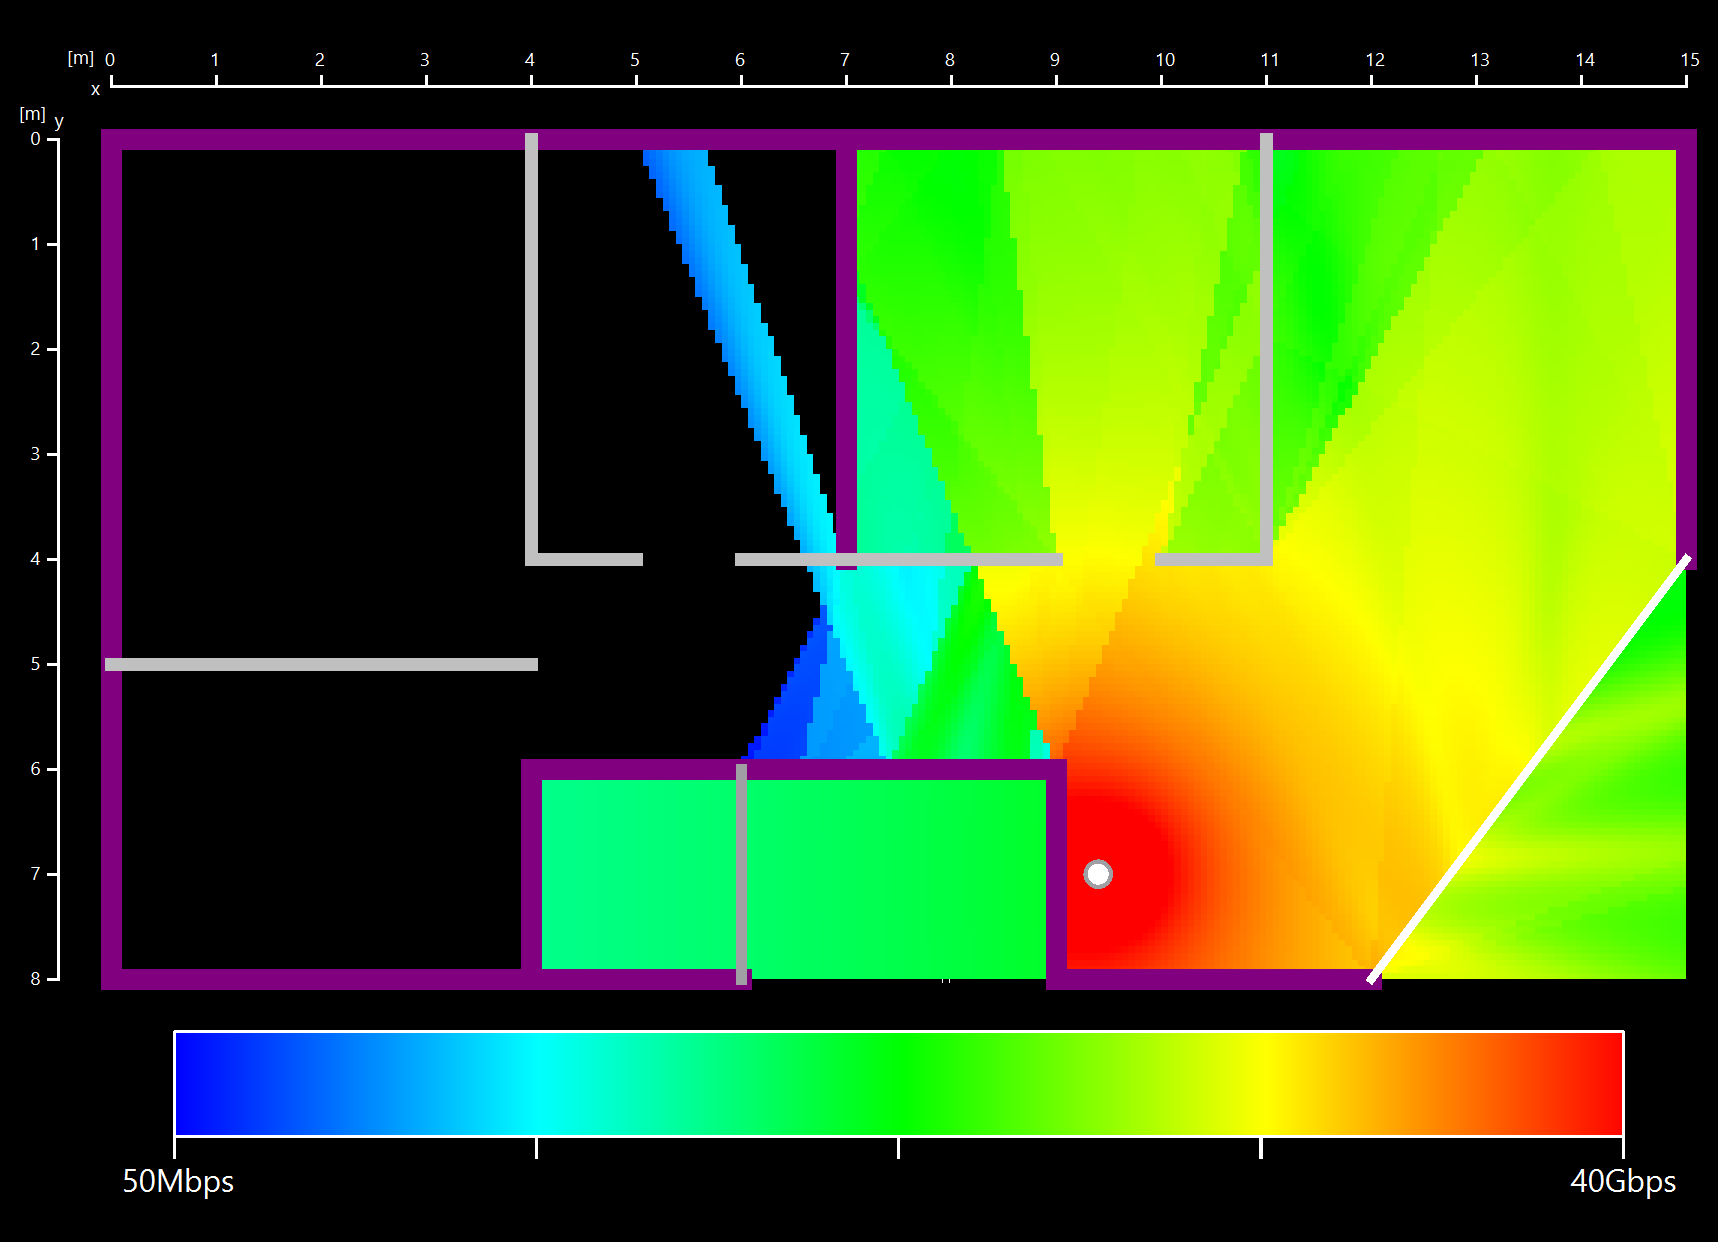
\includegraphics[width=0.7\textwidth]{latex/images/highres-without-lift.png}
    \caption{Couverture station de base salon, sans ascenseur}
    \label{fig:simu-emplacement-defaut-sansasc}
\end{figure}
\subsubsection{Avec ascenseur}

\begin{figure}[H]
    \centering
    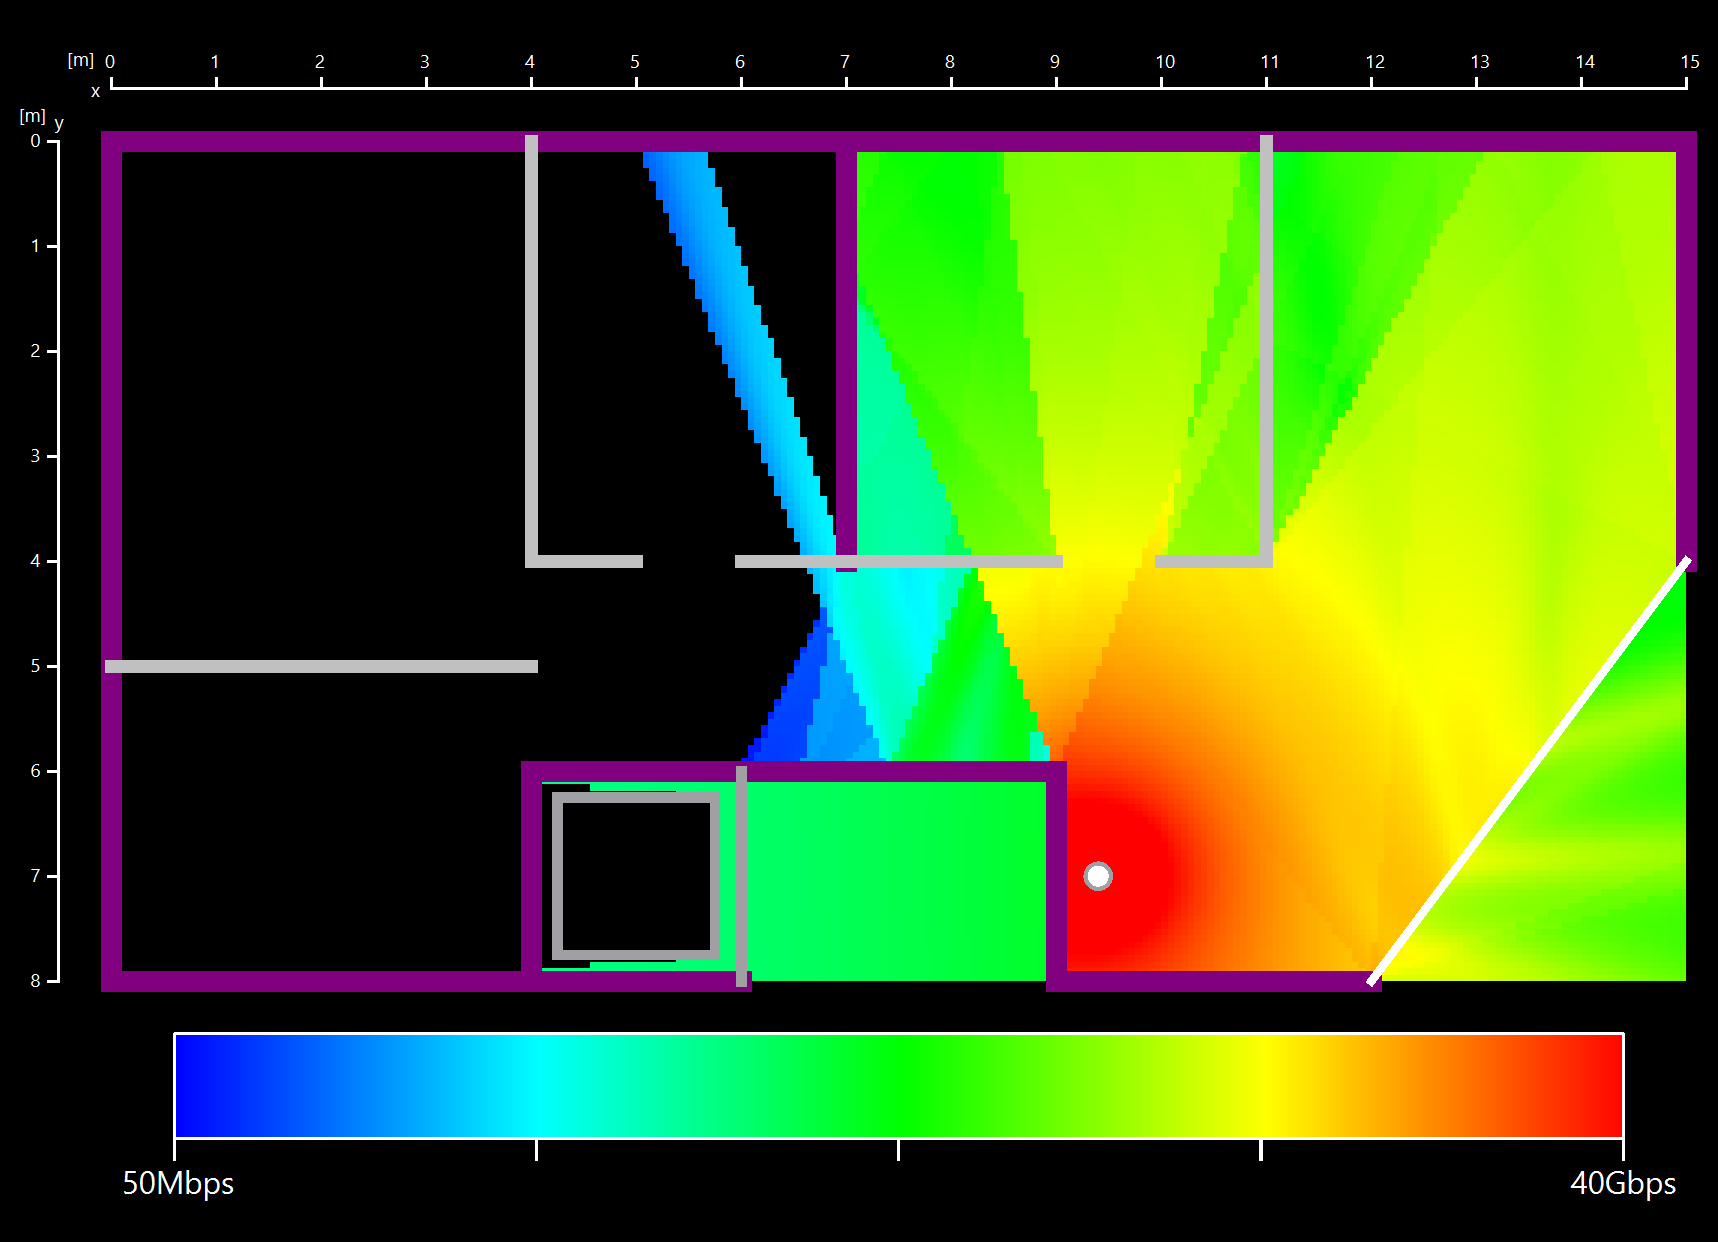
\includegraphics[width=0.7\textwidth]{latex/images/highres-with-lift.png}
    \caption{Couverture station de base salon, avec ascenseur}
    \label{fig:simu-emplacement-defaut-avecasc}
\end{figure}

\subsection{Emplacement couloir}
La station de base se trouve en (7 ; 5)m.

\subsubsection{Sans ascenseur}

\begin{figure}[H]
    \centering
    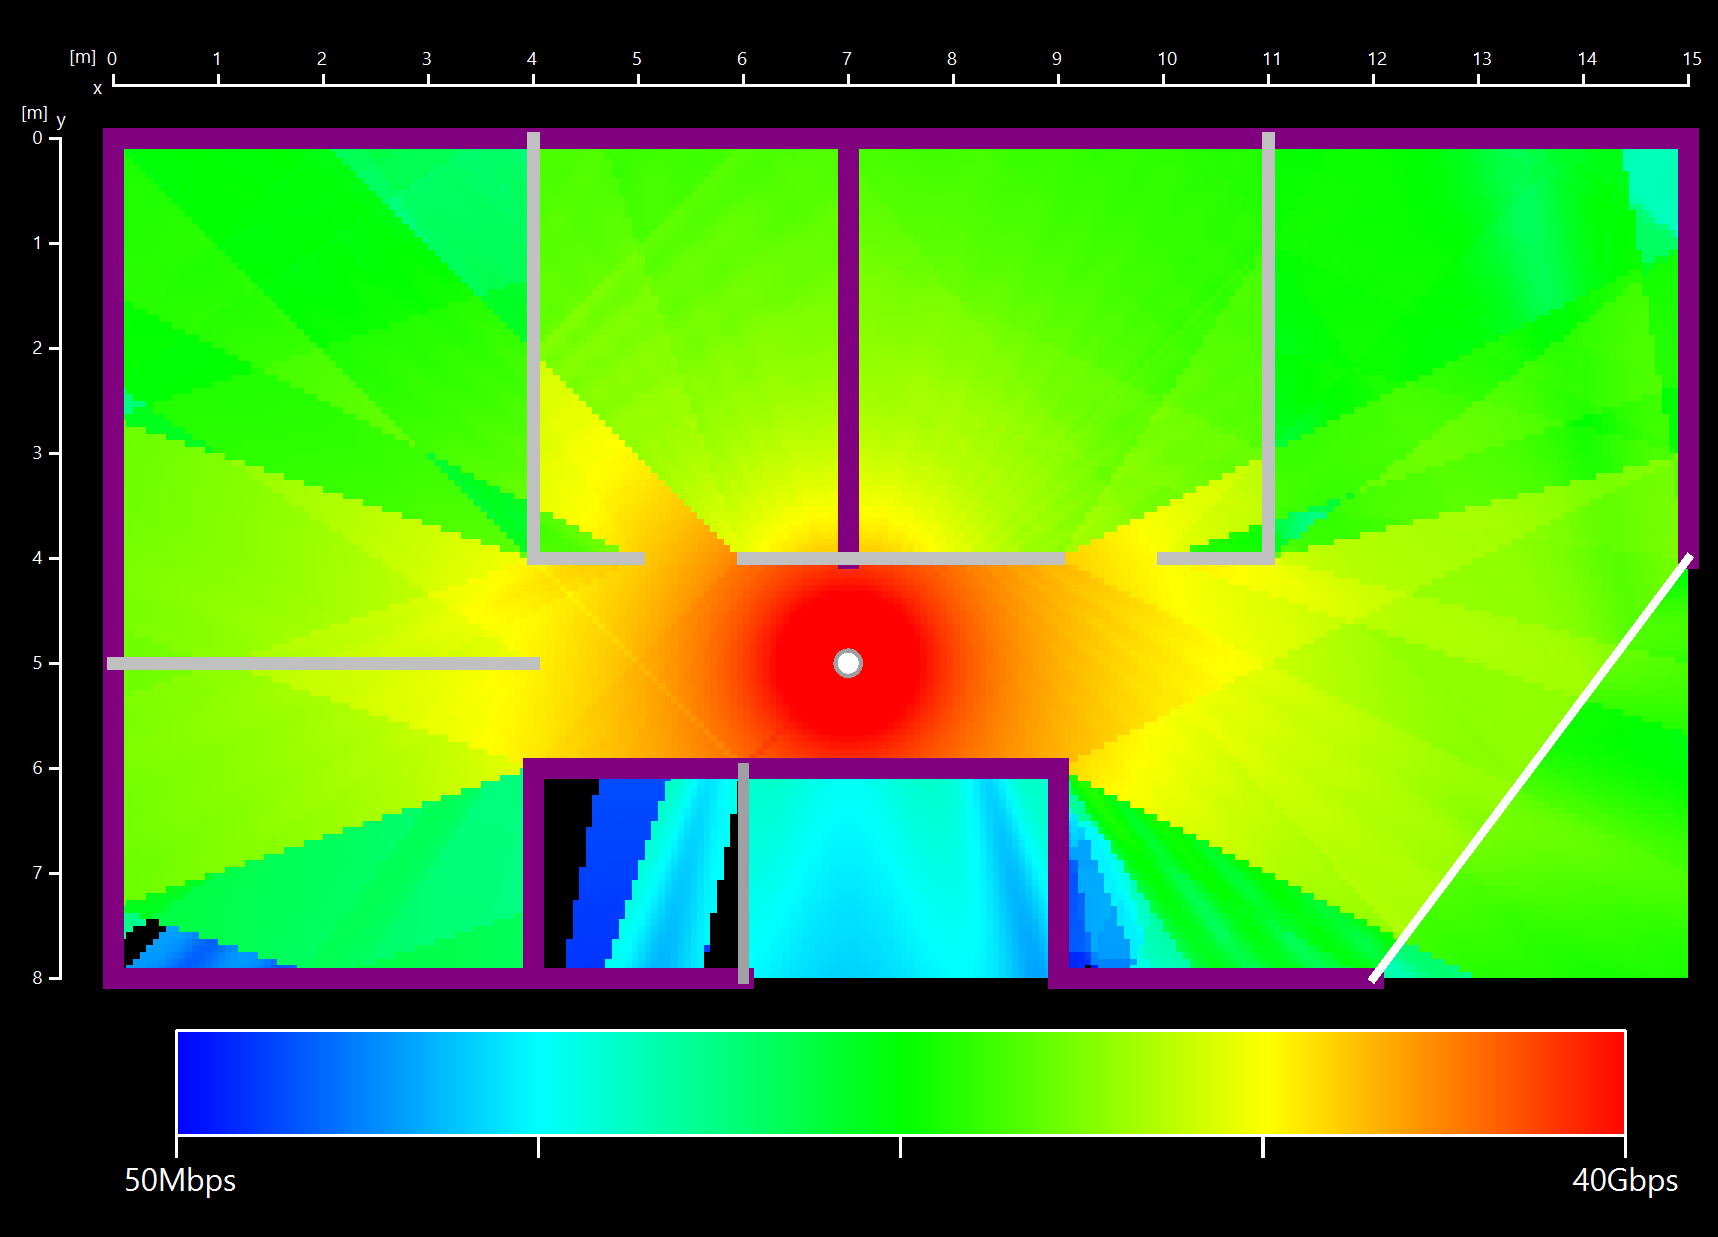
\includegraphics[width=0.7\textwidth]{latex/images/highres-couloir-without-lift.png}
    \caption{Couverture station de base couloir, sans ascenseur}
    \label{fig:simu-emplacement-couloir-sansasc}
\end{figure}
\subsubsection{Avec ascenseur}

\begin{figure}[H]
    \centering
    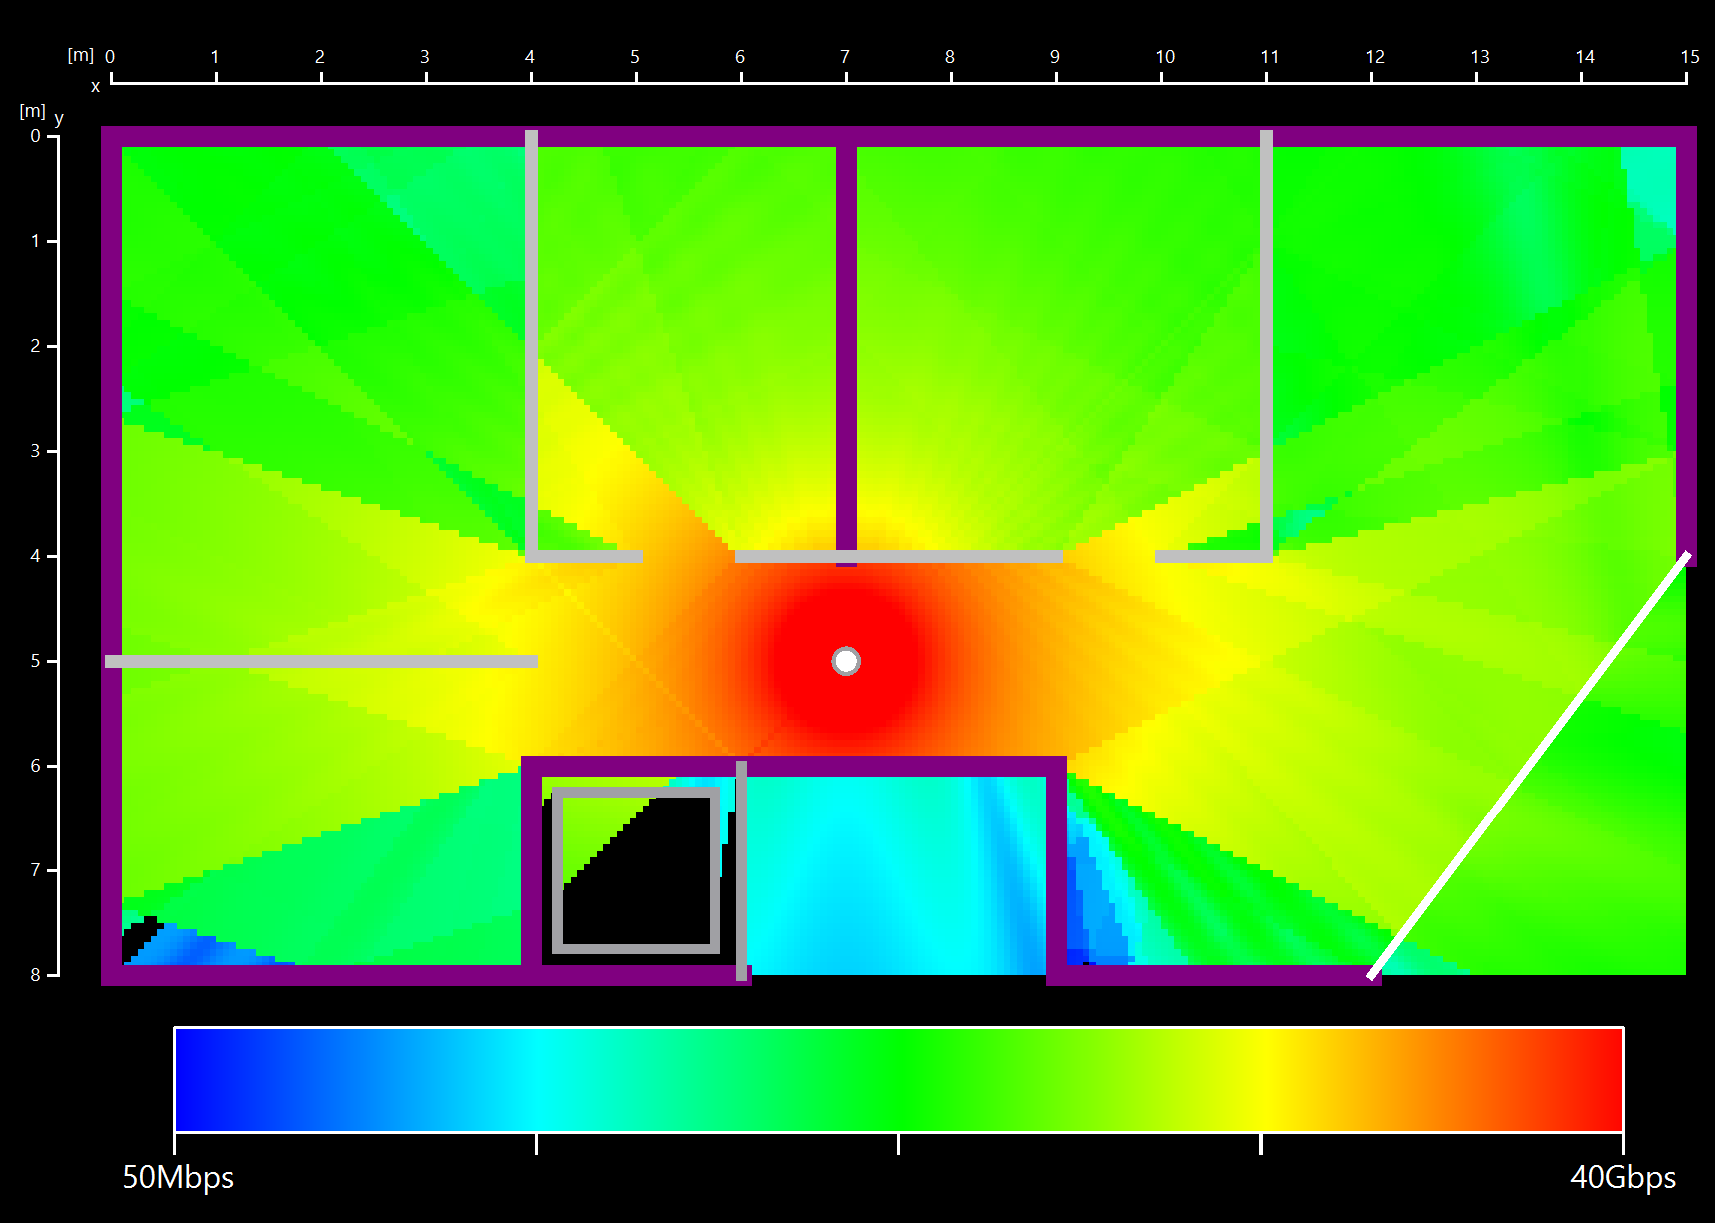
\includegraphics[width=0.7\textwidth]{latex/images/highres-couloir-with-lift.png}
    \caption{Couverture station de base couloir, avec ascenseur}
    \label{fig:simu-emplacement-couloir-avecasc}
\end{figure}


\subsection{Emplacement chambre 1}
La station de base se trouve en (0,5 ; 4)m.

\subsubsection{Sans ascenseur}

\begin{figure}[H]
    \centering
    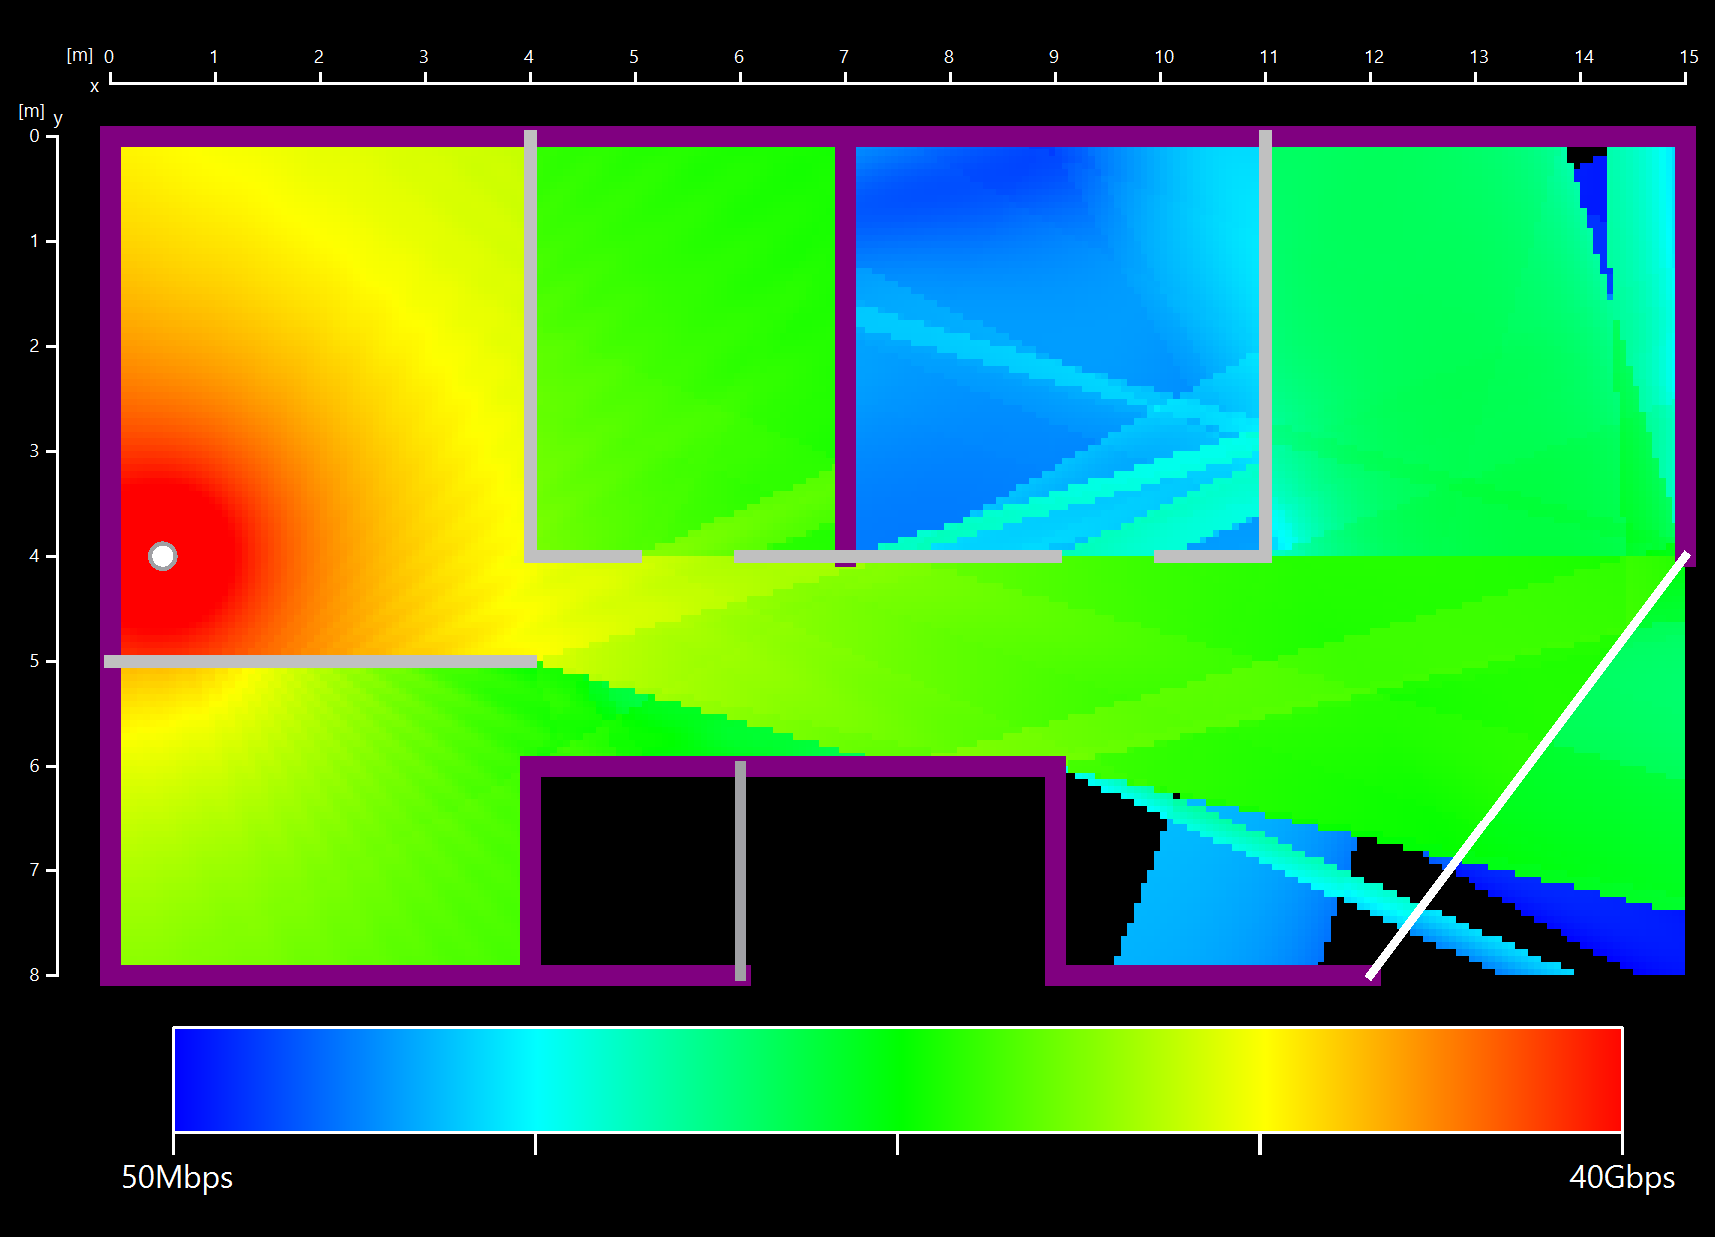
\includegraphics[width=0.7\textwidth]{latex/images/highres-chambre1-without-lift.png}
    \caption{Couverture station de base chambre 1, sans ascenseur}
    \label{fig:simu-emplacement-chambre1-sansasc}
\end{figure}
\subsubsection{Avec ascenseur}

\begin{figure}[H]
    \centering
    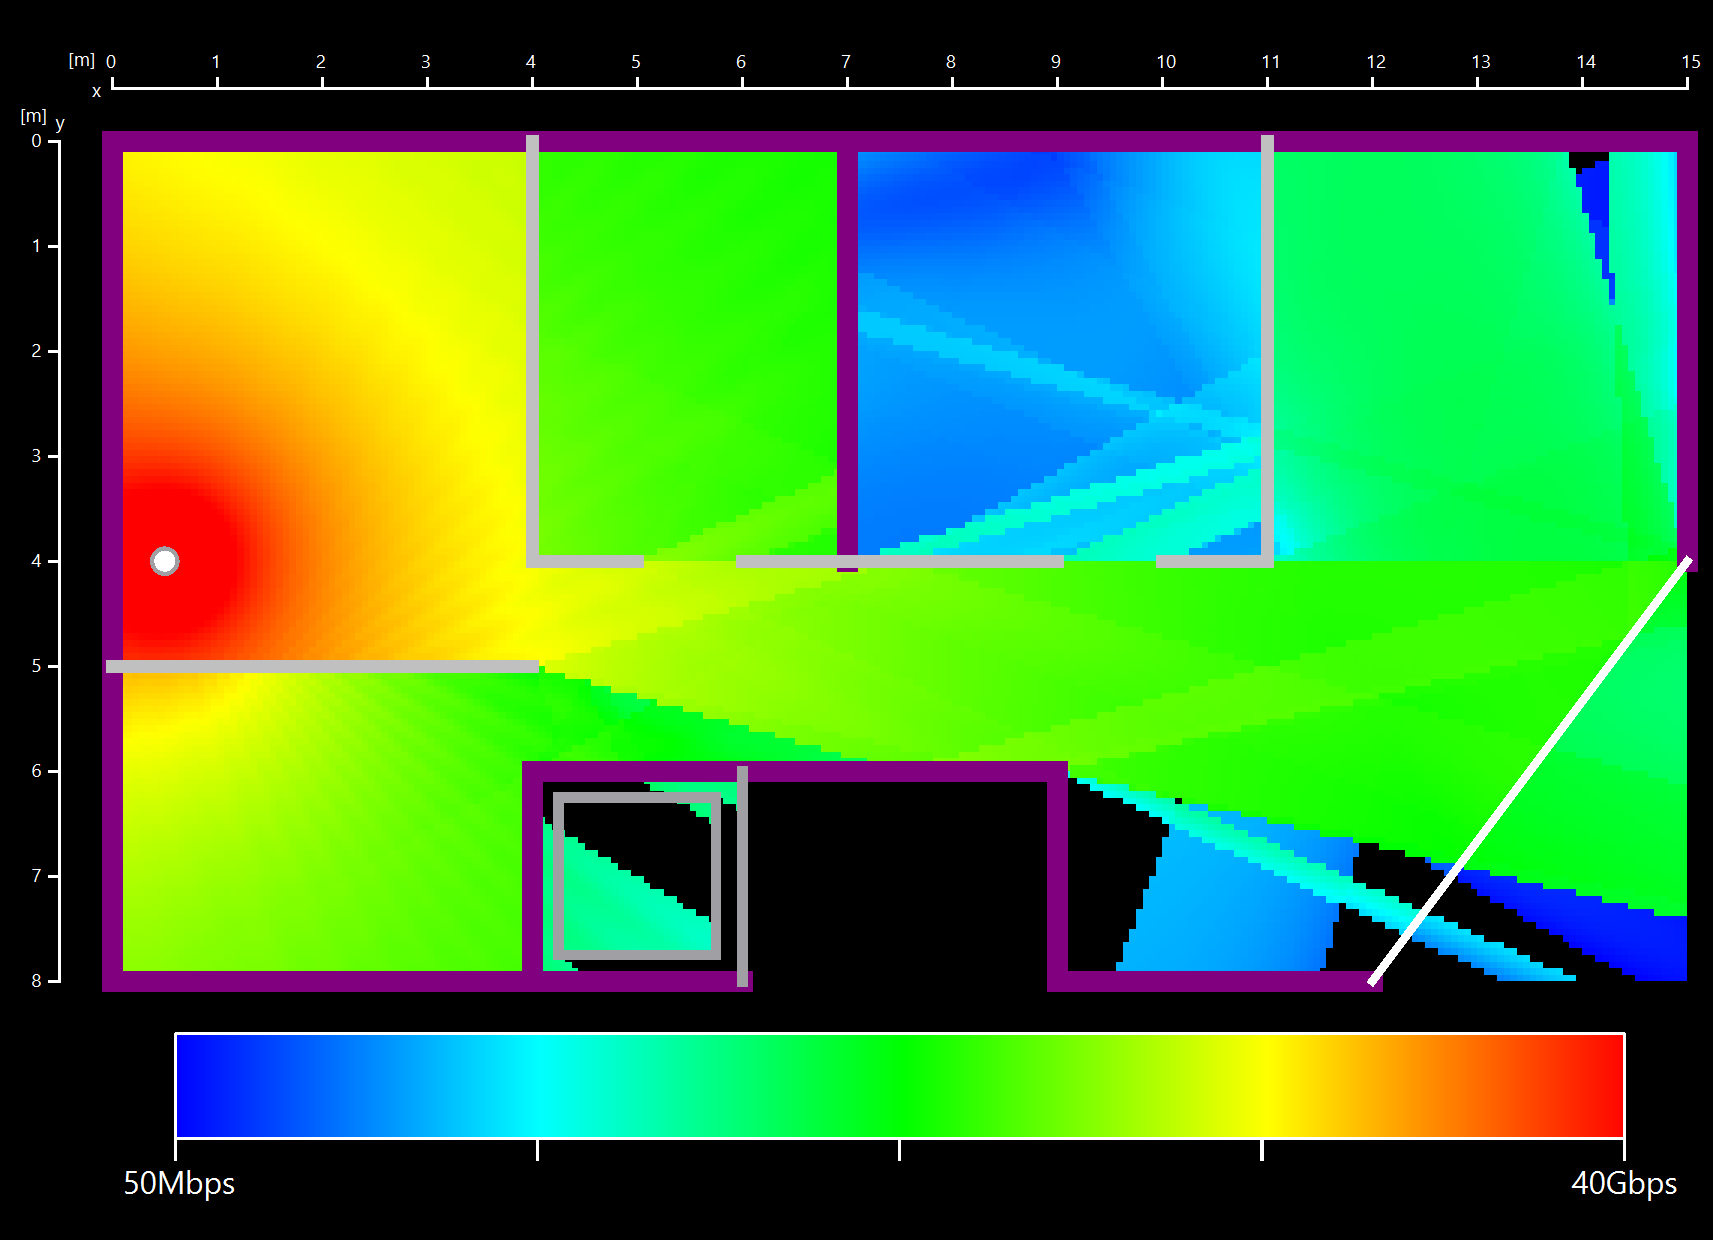
\includegraphics[width=0.7\textwidth]{latex/images/highres-chambre1-with-lift.png}
    \caption{Couverture station de base chambre 1, avec ascenseur}
    \label{fig:simu-emplacement-chambre1-avecasc}
\end{figure}


\section{Suggestions placement station de base}

Un emplacement dans le couloir au milieu de l'appartement offre une large couverture, dû à son placement central et à sa plus grande distance à tous les murs en béton.

Un emplacement au milieu d'une pièce est évidemment non favorable car loin de prises de courant et réseau, et nécessite aussi de placer la station de base au plafond ce qui engendre un travail supplémentaire lors de l'installation et un aspect esthétique moindre. Nous privilégions alors un emplacement proche d'un mur, sans doute sur un meuble, par soucis pratique.\\

L'emplacement par défaut du projet (9.4, 7)m est un emplacement réaliste et efficace car la station de base se trouve dans le salon de l'appartement, un lieu où est souvent le raccordement internet, et là où sont majoritairement utilisés les appareils sans-fil lors de besoins élevés en débit binaire (téléchargements, vidéos, etc). De plus, la cuisine et la salle à manger sont bien couvertes (deux autres pièces qui sont plus enclines à une utilisation du réseau Wi-Fi par les habitants, contrairement aux chambres et salle de bain).\\

\textbf{Pratiquement}, l'emplacement dans le salon semble être le meilleur choix.

\textbf{Théoriquement}, l'emplacement couloir semble offrir la meilleure couverture dans l'appartement.

\section{Critique de la simulation}
% TODO ?
% parler du fait que les murs sont rarement direct en béton (en général du placo par dessus), présence de meubles, absence de la diffraction, pas de beam-forming, etc...

Tout d'abord, on peut observer qu'un débit binaire non-nul est présent à côté de l'ascenseur, ainsi que dans sa cage ou dans lui-même. Ce résultat ne devrait pas se produire dû à la présence d'épais murs en béton ainsi que de la ou des parois métalliques constituant l'ascenseur. Cette erreur a malheureusement une origine inconnue, il se peut qu'elle survienne à cause d'un bug des coins des murs, où des ondes passeraient.\\

Ensuite, cette simulation repose sur de nombreuses simplifications et approximations. En effet, l'appartement ne présente pas d'obstacle de type meubles, ne possède aucune autre fenêtre (en plus de la baie vitrée oblique), des murs en béton sont normalement recouverts d'une couche de plâtre (affectant alors la réflexion différemment du béton). 

De plus, la simulation considère une antenne parfaitement omnidirectionnelle dans le plan étudié. 

Enfin, la simulation ne prend pas en compte la diffraction, et ignore les technologies maintenant très répandues dans les antennes Wi-Fi tel que le \textit{beam-forming} ou encore le \textit{MIMO}.
